\chapter[Planejamento]{Planejamento}
\label{cap:planejamento}

Nesta seção, será descrito o planejamento do projeto.

\section[Escolha do equipamento]{Escolha do equipamento}

Para o desenvolvimento do projeto, foram disponibilizados, pela instituição CEFET-MG, dois manipuladores robóticos e diversos dispositivos que podem ser utilizados para seu controle.

\subsection[Manipuladores]{Manipuladores}

Os principais elementos deste trabalho são os manipuladores robóticos, portanto foi feito inicialmente um estudo sobre seu funcionamento e sobre como podem ser controlados.

Os manipuladores disponibilizados possuem diferenças físicas entre si, portanto o controle de cada um deles deve ser programado de forma independente.
Para diferenciá-los, serão denominados Manipulador Azul e Manipulador Preto.
A seguir, serão descritos os principais aspectos de cada um deles.

\begin{figure}[H]
    \begin{minipage}{.5\textwidth}
        \centering
        \caption{Manipulador Robótico Azul}
        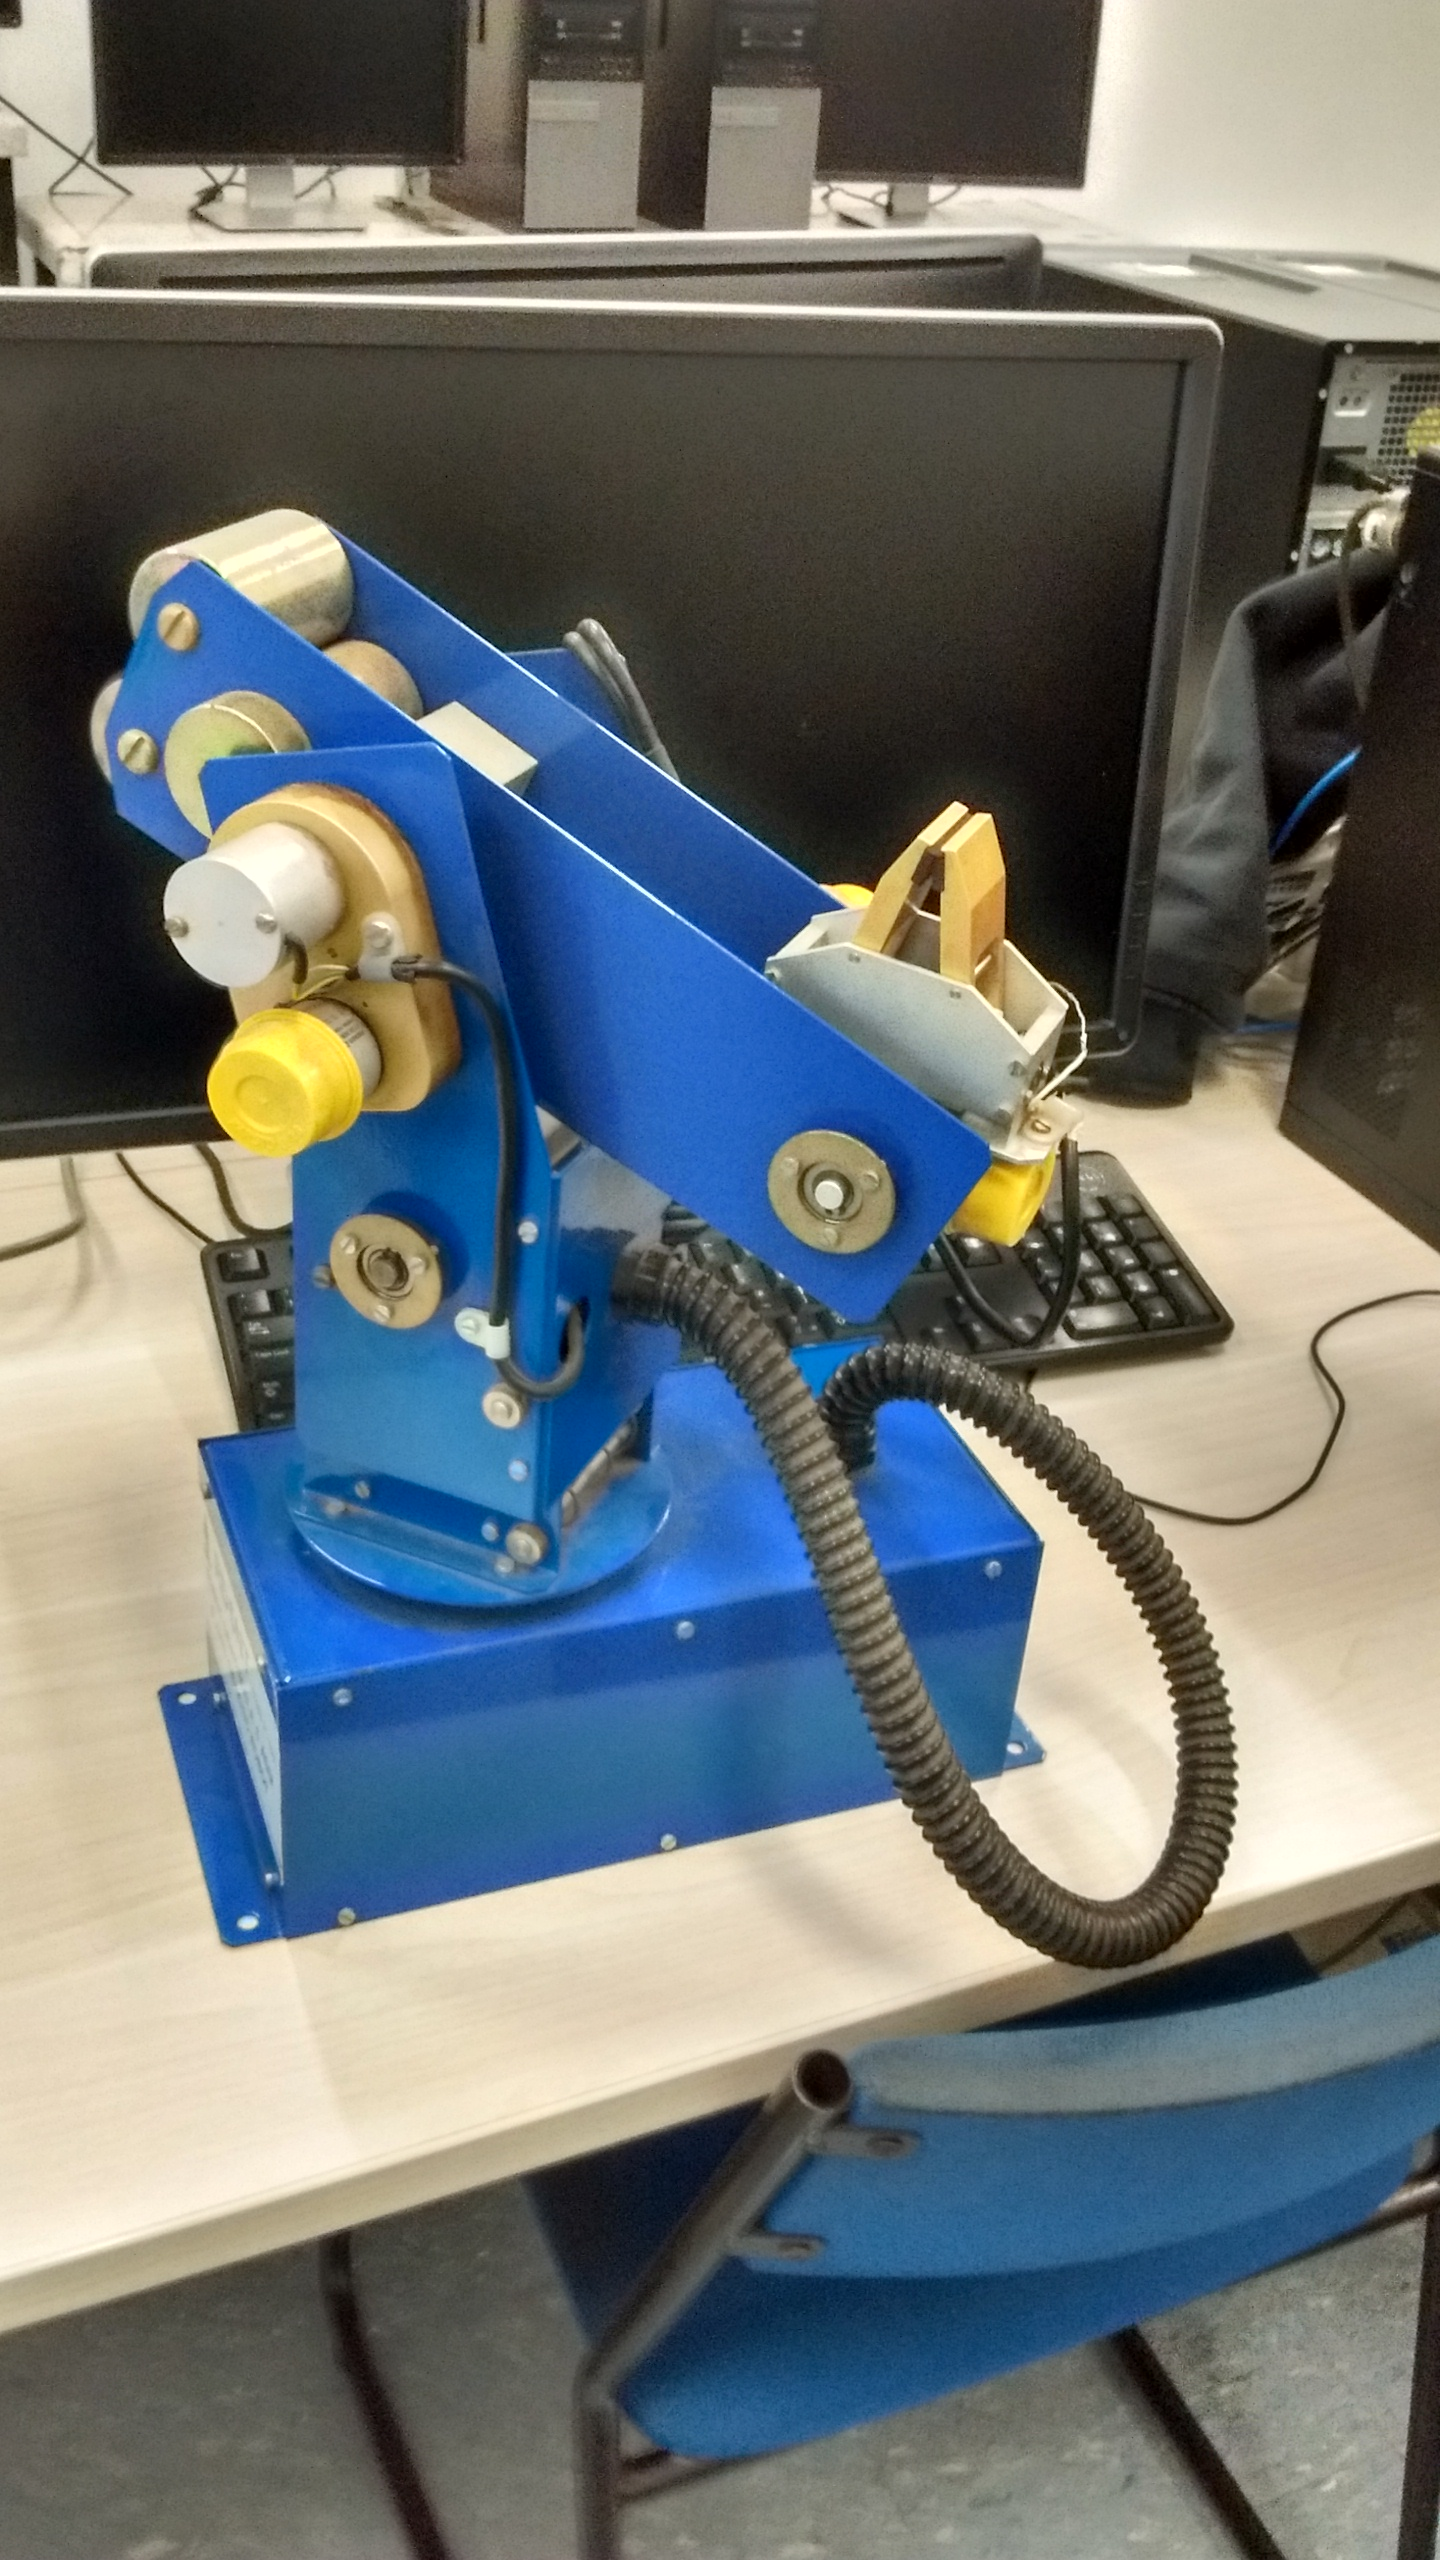
\includegraphics[keepaspectratio=true, width=0.9\linewidth]
            {img/foto-manipulador-azul.jpg}
        \fonte{http://arquivo.eng.br/robotica}
        \label{fig:fotoManipuladorAzul}
    \end{minipage}%
    \begin{minipage}{.5\textwidth}
        \centering
        \caption{Manipulador Robótico Preto}
        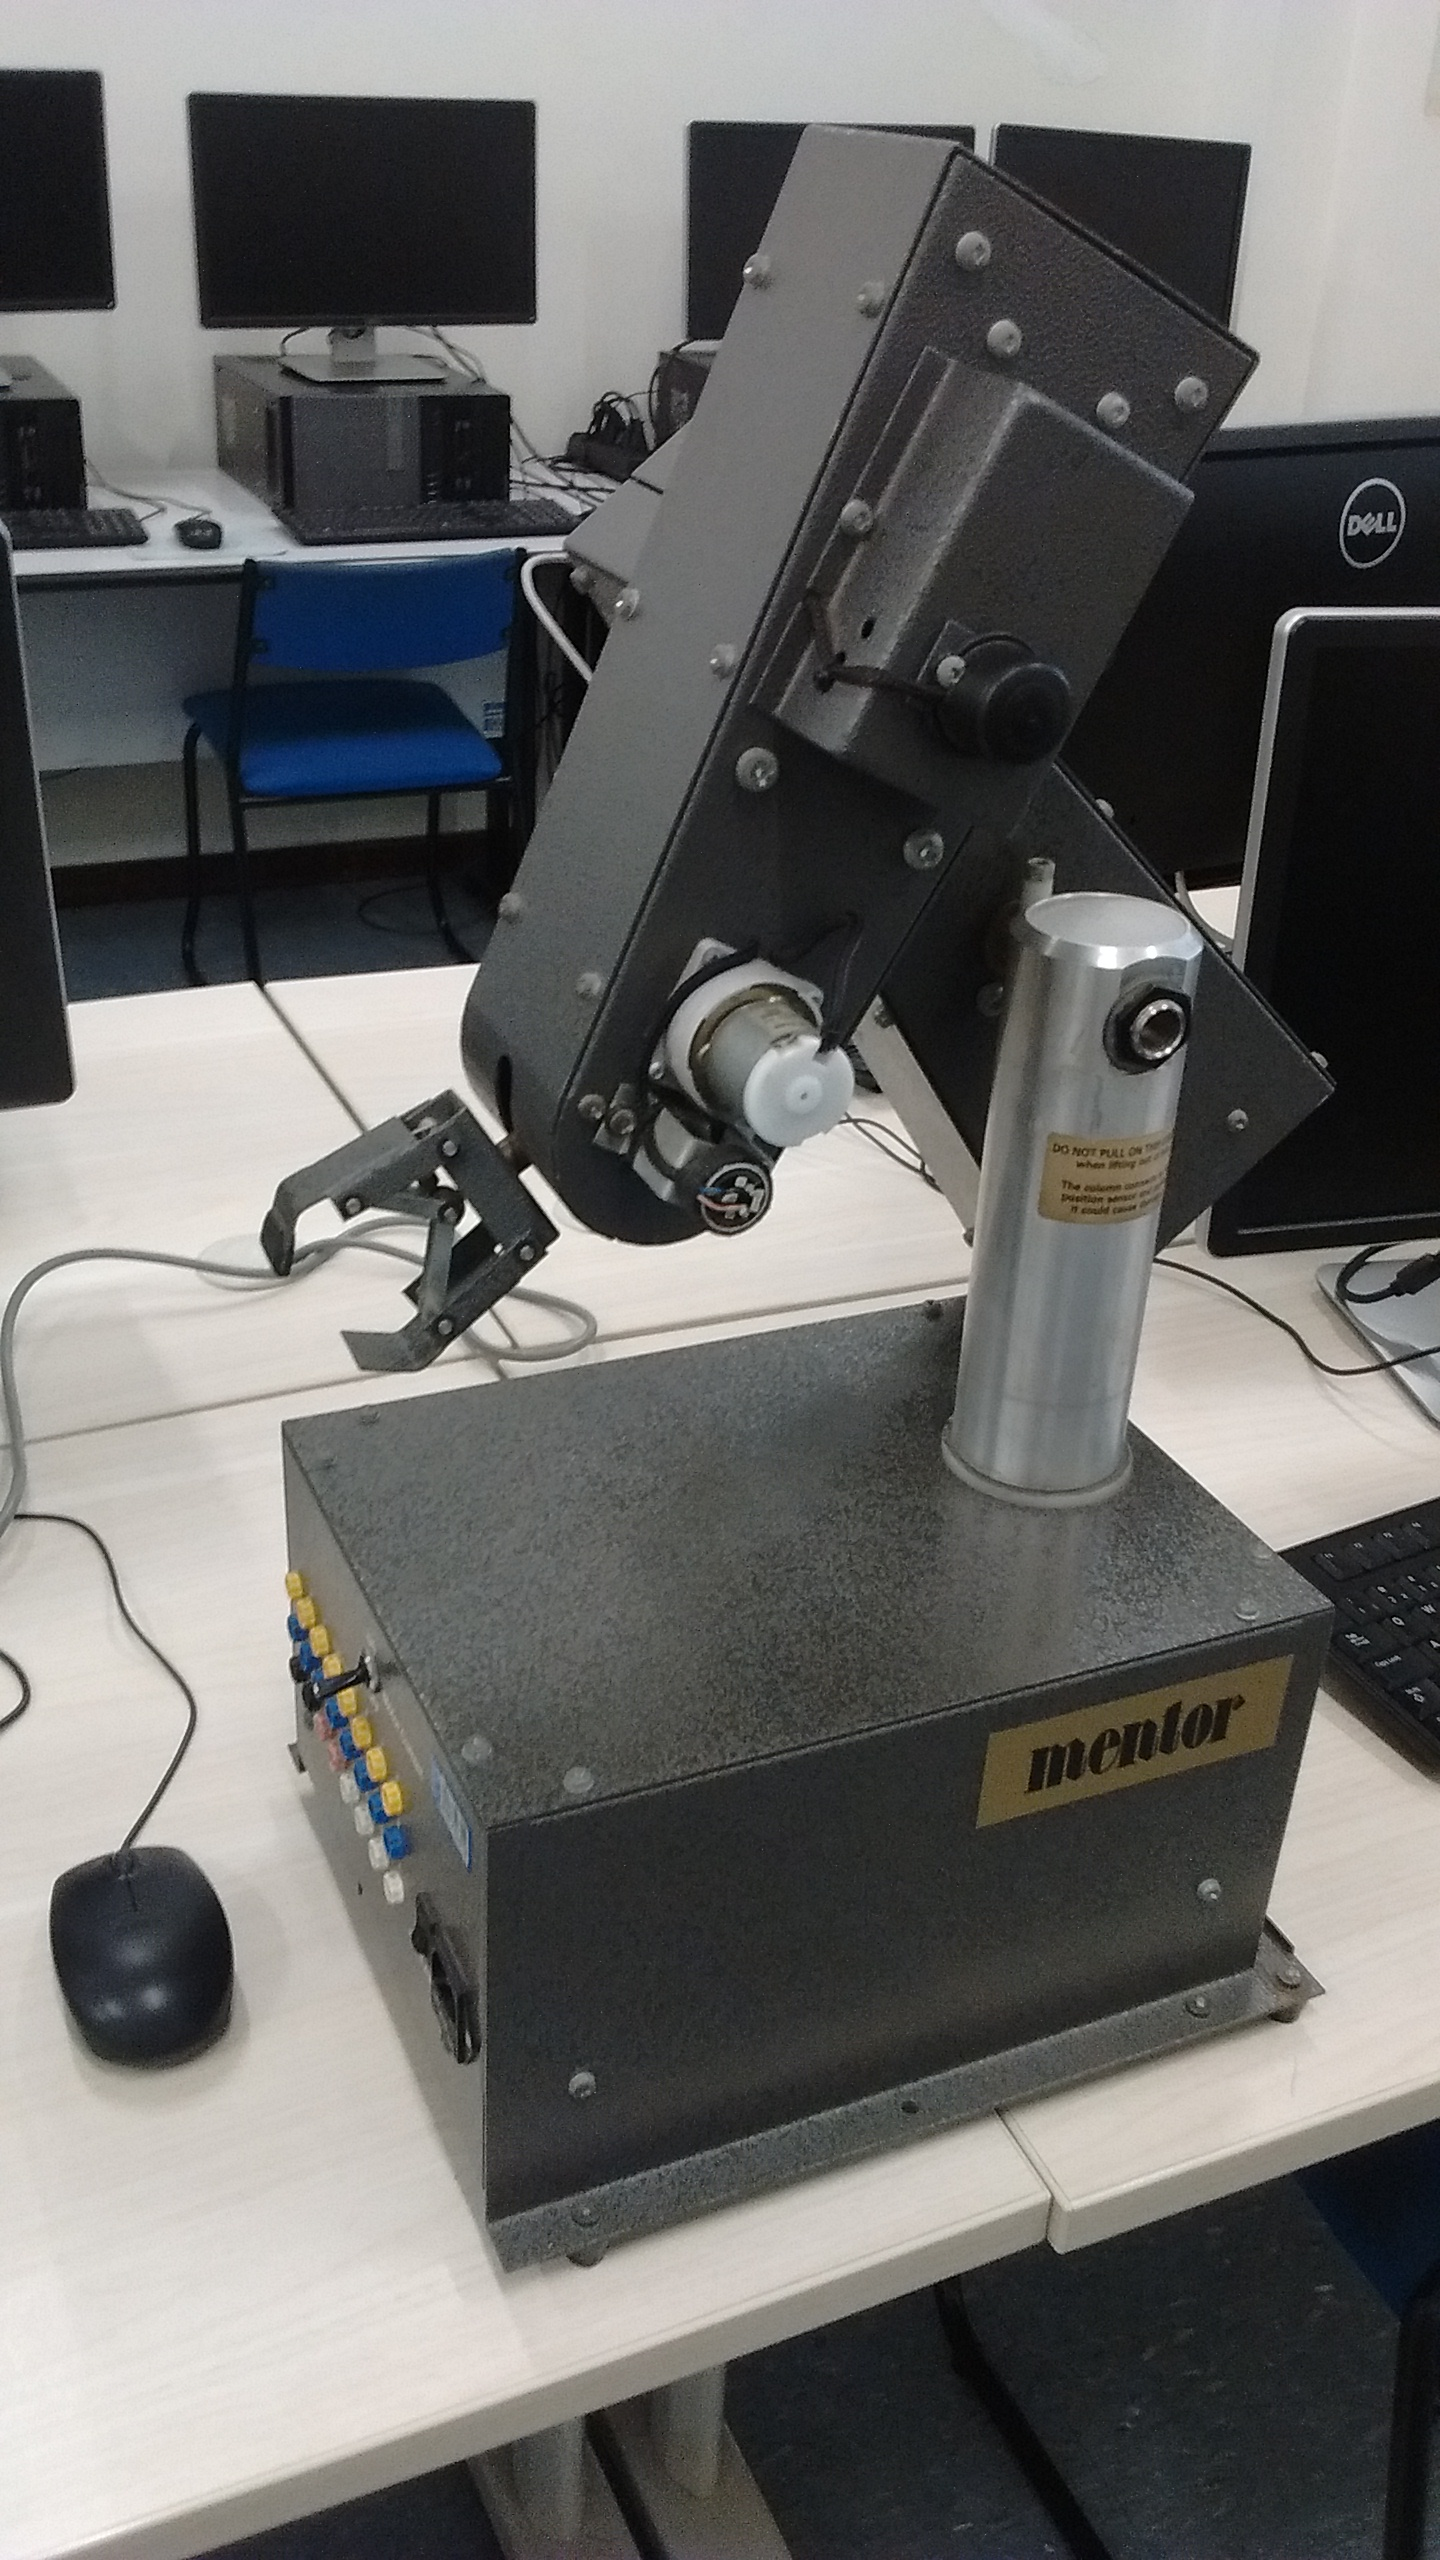
\includegraphics[keepaspectratio=true, width=0.9\linewidth]
            {img/foto-manipulador-preto.jpg}
        \fonte{http://arquivo.eng.br/robotica}
        \label{fig:fotoManipuladorPreto}
    \end{minipage}
\end{figure}

\subsection[Manete para os jogadores]{Manete para os jogadores}

Para que os jogadores possam interagir com os manipuladores, foi utilizado uma manete que possui dois \textit{joysticks} e um botão integrado a cada \textit{joystick}.
Cada jogador possui uma manete para mover seu manipulador nos eixos X e Y, e selecionar a peça que deseja mover.

\begin{figure}[H]
    \centering
    \caption{Manete para os jogadores}
    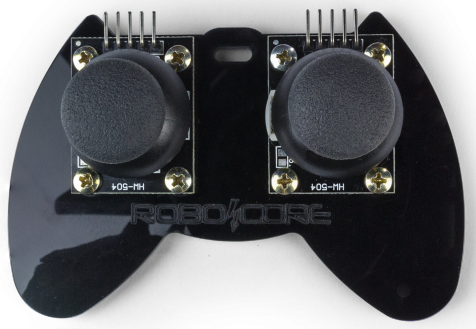
\includegraphics[keepaspectratio=true, width=0.5\textwidth]
    	{img/foto-controle-jogadores.png}
    \fonte{https://www.robocore.net/acessorios-robocore/controle-batpad}
    \label{fig:fotoManeteJogadores}
\end{figure}

\subsection[Microcontrolador]{Microcontrolador}

Para realizar a leitura dos dados das manetes e enviar os comandos para os manipuladores, foi utilizado um microcontrolador Arduino Uno.
Este dispositivo deve receber sinais analógicos provenientes dos \textit{joysticks}, receber sinais digitais provenientes dos botões nos controles, receber sinais analógicos que indicam as posições dos manipuladores e enviar sinais digitais do tipo PWM para os motores dos manipuladores.

\begin{figure}[H]
    \centering
    \caption{Microcontrolador Arduino Uno}
    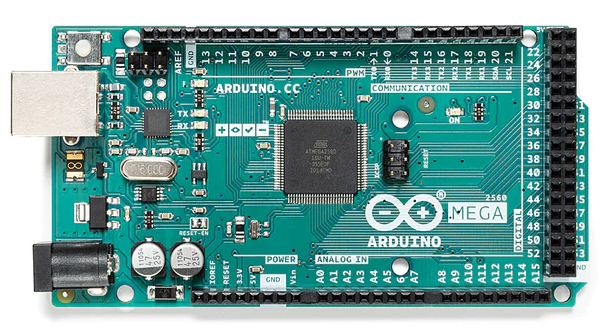
\includegraphics[keepaspectratio=true, width=0.5\textwidth]
    	{img/foto-arduino.png}
    \fonte{https://store-usa.arduino.cc/products/arduino-uno-rev3}
    \label{fig:fotoArduino}
\end{figure}

\section[Projeto do sistema]{Projeto do sistema}

Com todos os equipamentos definidos, foi feito o projeto do sistema, que consiste na definição de como os dispositivos serão interligados e como o sistema irá funcionar.

O microcontrolador Arduino é a base do sistema, pois ele realiza a interligação entre os outros componentes.
As manetes são conectadas ao Arduino por meio de 10 cabos cada, sendo 5 para cada \textit{joystick}, com seu respectivo botão.
Os manipuladores são conectados ao Arduino por meio de 10 cabos cada, sendo 5 para a leitura de cada ângulo dos motores, e 5 para o controle desses.

A montagem do sistema é mostrada na Figura %\ref{fig:montagemSistema}.%

%Inserir figura%


